\documentclass{article}
\usepackage[utf8x]{inputenc}
\usepackage[english,russian]{babel}
\usepackage{geometry}
  \geometry{left=2cm}
  \geometry{right=1.5cm}
  \geometry{top=1cm}
  \geometry{bottom=2cm}
\usepackage{tikz}
\usepackage{multicol}
\usepackage{listings}
\usepackage{textcomp}

\begin{document}
\pagenumbering{gobble}

\lstset{
  language=C,                % choose the language of the code
  basicstyle=\linespread{1.1}\ttfamily,
  columns=fixed,
  fontadjust=true,
  basewidth=0.5em,
  keywordstyle=\color{blue}\bfseries,
  commentstyle=\color{gray},
  stringstyle=\ttfamily\color{orange!50!black},
  showstringspaces=false,
  %numbers=false,                   % where to put the line-numbers
  numbersep=5pt,
  numberstyle=\tiny\color{black},
  numberfirstline=true,
  stepnumber=1,                   % the step between two line-numbers.        
  numbersep=10pt,                  % how far the line-numbers are from the code
  backgroundcolor=\color{white},  % choose the background color. You must add \usepackage{color}
  showstringspaces=false,         % underline spaces within strings
  captionpos=b,                   % sets the caption-position to bottom
  breaklines=true,                % sets automatic line breaking
  breakatwhitespace=true,         % sets if automatic breaks should only happen at whitespace
  xleftmargin=.2in,
  extendedchars=\true,
  keepspaces = true,
  upquote=true,
}
\lstset{literate=%
   *{0}{{{\color{red!20!violet}0}}}1
    {1}{{{\color{red!20!violet}1}}}1
    {2}{{{\color{red!20!violet}2}}}1
    {3}{{{\color{red!20!violet}3}}}1
    {4}{{{\color{red!20!violet}4}}}1
    {5}{{{\color{red!20!violet}5}}}1
    {6}{{{\color{red!20!violet}6}}}1
    {7}{{{\color{red!20!violet}7}}}1
    {8}{{{\color{red!20!violet}8}}}1
    {9}{{{\color{red!20!violet}9}}}1
}

\renewcommand{\thesubsection}{\arabic{subsection}}
\makeatletter
\def\@seccntformat#1{\@ifundefined{#1@cntformat}%
   {\csname the#1\endcsname\quad}%    default
   {\csname #1@cntformat\endcsname}}% enable individual control
\newcommand\section@cntformat{}     % section level 
\newcommand\subsection@cntformat{Задача \thesubsection.\space} % subsection level
\newcommand\subsubsection@cntformat{\thesubsubsection.\space} % subsubsection level
\makeatother


\title{Семинар \#4: Часть 1: Указатели. Домашнее задание. \vspace{-5ex}}\date{}\maketitle


\subsection{Одна строка}
Решения всех подзадач этой задачи -- одна строка. Вам нужно создать файл в формате \texttt{.txt} и, используя любой текстовый редактор, записать в него ответы на все подзадачи. После этого, файл нужно поместить в ваш репозиторий на github.

\begin{enumerate}
\item В следующей программе создайте указатель \texttt{p} и инициализируйте его адресом переменной \texttt{a}:
\begin{lstlisting}
int main() 
{
    int a = 10;
    // Тут нужно написать 1 строку кода
}
\end{lstlisting}

\item Создайте указатель \texttt{p} и инициализируйте его адресом переменной \texttt{a}:
\begin{lstlisting}
int main() 
{
    float a = 1.1;
    // Тут нужно написать 1 строку кода
}
\end{lstlisting}


\item Создайте указатель \texttt{p} и сделайте так, чтобы он указывал на первый элемент массива (индекс \texttt{0}):
\begin{lstlisting}
int main() 
{
    int array[5] = {10, 20, 30, 40, 50};
    // Тут нужно написать 1 строку кода
}
\end{lstlisting}


\item Создайте указатель \texttt{p} и сделайте так, чтобы он указывал на символ \texttt{'A'}  из строки \texttt{str}:
\begin{lstlisting}
int main() 
{
    char str[20] = "Sapere Aude";
    // Тут нужно написать 1 строку кода
}
\end{lstlisting}

\item Создайте указатель \texttt{q} и инициализируйте его адресом переменной \texttt{p}:
\begin{lstlisting}
int main() 
{
    int a = 10;
    int* p = &a;
    // Тут нужно написать 1 строку кода
}
\end{lstlisting}

\newpage
\item В следующей программе удвойте значение переменной \texttt{a}, используя только указатель \texttt{p}. Нужно использовать указатель \texttt{p}. Переменную \texttt{a} использовать нельзя.
\begin{multicols}{2}\noindent
\begin{lstlisting}
#include <stdio.h>
int main() 
{
    int a = 10;
    int* p = &a;
    // Тут нужно написать 1 строку кода
    
    printf("%i\n", a);
}
\end{lstlisting}
\vfill \null    
\columnbreak
\vfill \null 
\begin{center}
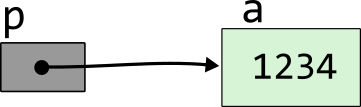
\includegraphics[scale=1]{../images/pointer_schemes/pointer_to_int.png}
\end{center}
\end{multicols}


\item Переведите символ, хранящийся в переменной \texttt{a} в верхний регистр, используя только указатель \texttt{p}. Нужно использовать только указатель \texttt{p}. Переменную \texttt{a} использовать нельзя.
\begin{multicols}{2}\noindent
\begin{lstlisting}
#include <stdio.h>
int main() 
{
    char a = 't';
    char* p = &a;
    // Тут нужно написать 1 строку кода
    
    printf("%c\n", a);
}
\end{lstlisting}
\vfill \null    
\columnbreak
\vfill \null 
\begin{center}
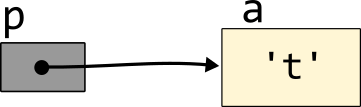
\includegraphics[scale=1]{../images/pointer_schemes/pointer_to_char.png}
\end{center}
\end{multicols}


\item В следующей программе добавьте \texttt{1} к четвёртому элементу массива, используя только указатель \texttt{p} на первый элемент. Нужно использовать только указатель \texttt{p}. Массив \texttt{a} использовать нельзя.
\begin{multicols}{2}\noindent
\begin{lstlisting}
#include <stdio.h>
int main() 
{
    int a[5] = {10, 20, 30, 40, 50};
    int* p = &a[0];
    // Тут нужно написать 1 строку кода
    
    for (int i = 0; i < 5; ++i) 
        printf("%i ", a[i]);
}
\end{lstlisting}
\vfill \null    
\columnbreak
\vfill \null 
\begin{center}
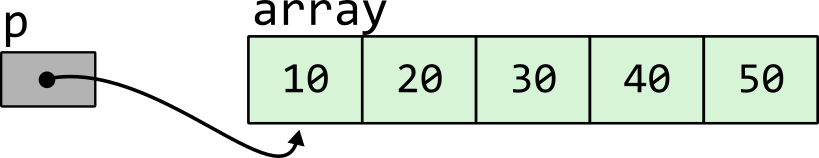
\includegraphics[scale=0.8]{../images/pointer_schemes/pointer_to_int_array.png}
\end{center}
\end{multicols}




\newpage$•$
\item В следующей программе используйте указатель на четвёртый элемент массива(\texttt{p}), чтобы добавить \texttt{1} к первому элементу массива. Нужно использовать только указатель \texttt{p}. Массив \texttt{a} использовать нельзя.
\begin{multicols}{2}\noindent
\begin{lstlisting}
#include <stdio.h>
int main() 
{
    int a[5] = {10, 20, 30, 40, 50};
    int* p = &a[3];
    // Тут нужно написать 1 строку кода
    
    for (int i = 0; i < 5; ++i)
        printf("%i ", a[i]);
}
\end{lstlisting}
\vfill \null    
\columnbreak
\vfill \null 
\begin{center}
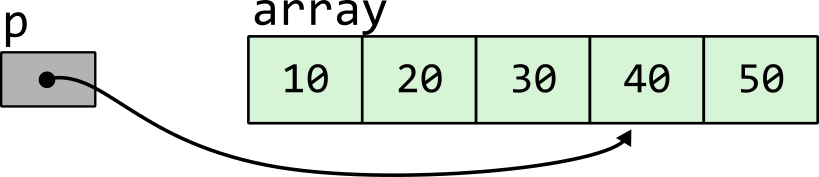
\includegraphics[scale=0.8]{../images/pointer_schemes/pointer_to_int_array_index4.png}
\end{center}
\end{multicols}


\item В следующей программе переведите в верхний регистр все буквы строки, используя только указатель \texttt{p}. Нужно использовать только указатель \texttt{p}. Строку \texttt{str} использовать нельзя. Решение -- 1 цикл (2 строки кода).
\begin{multicols}{2}
\noindent
\begin{lstlisting}
#include <stdio.h>
int main() 
{
    char str[] = "sapere aude";
    char* p = &str[0];
    // Тут нужно написать 2 строки кода

    printf("%s\n", str);
}
\end{lstlisting}
\begin{center}
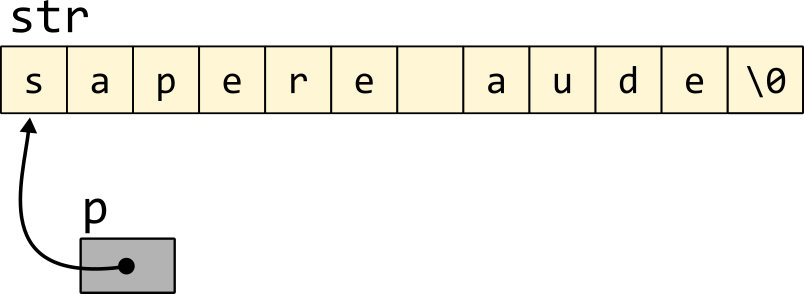
\includegraphics[scale=0.8]{../images/pointer_schemes/pointer_to_char_array.png}
\end{center}
\end{multicols}


\item Удвойте значение переменной \texttt{a}, используя только указатель \texttt{q}. Нужно использовать только указатель \texttt{q}. Использовать переменные \texttt{a} и \texttt{p} нельзя.
\begin{multicols}{2}
\noindent
\begin{lstlisting}
#include <stdio.h>
int main() 
{
    int a = 10;
    int* p = &a;
    int** q = &p;
    // Тут нужно написать 1 строку кода
    
    printf("%i\n", a);
}
\end{lstlisting}

\vfill \null    
\columnbreak
\vfill \null 

\begin{center}
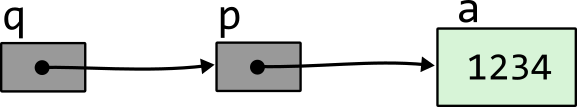
\includegraphics[scale=1]{../images/pointer_schemes/pointer_to_pointer_to_int.png}
\end{center}
\end{multicols}


\end{enumerate}








\newpage
\subsection{Указатель в массиве}
Решения всех подзадач этой задачи -- одно число. Вам нужно создать файл в формате \texttt{.txt} и, используя любой текстовый редактор, записать в него ответы на все подзадачи. После этого, файл нужно поместить в ваш репозиторий на github.

Пусть есть массив и указатель на 4-й элемент этого массива:
\begin{lstlisting}
int numbers[6] = {4, 8, 15, 16, 23, 42};
int* p = &numbers[3];
\end{lstlisting}

\begin{center}
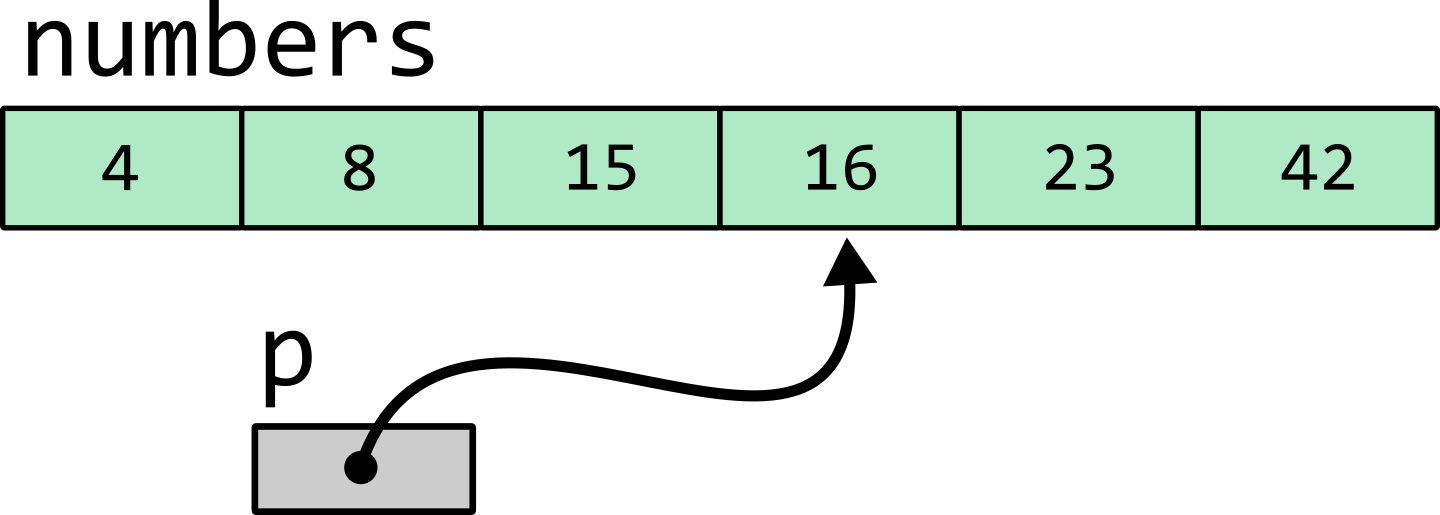
\includegraphics[scale=0.7]{../images/pointer_task_arithmetics.png}
\end{center}

Чему равны следующие выражения:
\begin{multicols}{3}
\begin{enumerate}
\item \begin{verbatim} numbers[5] \end{verbatim}
\item \begin{verbatim} *p \end{verbatim}
\item \begin{verbatim} *(p+1) \end{verbatim}
\item \begin{verbatim} *(p-2) \end{verbatim}
\item \begin{verbatim} p[0] \end{verbatim}
\item \begin{verbatim} p[1] \end{verbatim}
\item \begin{verbatim} p[-2] \end{verbatim}
\item \begin{verbatim} *numbers \end{verbatim}
\item \begin{verbatim} *(numbers+5) \end{verbatim}
\item \begin{verbatim} p - numbers \end{verbatim}
\item \begin{verbatim} (short*)p - (short*)numbers \end{verbatim}
\item \begin{verbatim} (char*)p - (char*)numbers \end{verbatim}
\end{enumerate}
\end{multicols}


\subsection{Куб по указателю}
Напишите функцию \texttt{cube}, которая будет принимать на вход адрес некоторой переменной типа \texttt{float}. 
\begin{lstlisting}
void cube(float* px)
\end{lstlisting}

Функция должна возводиить в куб переменную, чей адрес хранит входящий указатель. Вызовите эту функцию из \texttt{main} и протестируйте её.

\subsection{Умножение массива на 2}
Напишите функцию
\begin{lstlisting}
void mult2(int* p, size_t n)
\end{lstlisting}
которая будет принимать указатель на первый элемент некоторого массива \texttt{p} и целое число \texttt{n}, равное размеру этого массива. Функция должна увеличивать все элементы массива в 2 раза.
Решите эту задачу в двух вариантах:
\begin{enumerate}
\item[a.] К указателю можно применять только оператор сложения \texttt{+} и оператор разыменования \texttt{*}.
\item[b.] К указателю можно применять только оператор квадратные скобки \texttt{[]}.
\end{enumerate}



\subsection{Квадратное уравнение}
Напишите функцию
\begin{lstlisting}
int solve_quadratic(double a, double b, double c, double* px1, double* px2)
\end{lstlisting}
которая должна решать квадратное уравнение с коэффициентами \texttt{a}, \texttt{b} и \texttt{c}. Результат функция должна записывать по адресам \texttt{px1} и \texttt{px2}. Функция должна возвращать:
\begin{itemize}
\item \texttt{0} - если корней нет. По адресам \texttt{px1} и \texttt{px2} ничего записывать в этом случае не надо.
\item \texttt{1} - если есть один корень. Его нужно записать по адресу \texttt{px1}.
\item \texttt{2} - если есть два корня. Их нужно записать по адресам \texttt{px1} и \texttt{px2}.
\end{itemize}
Все сравнения делать с точностью \texttt{eps = 1e-10}.

\subsection{Изменить символы}
Напишите функцию
\begin{lstlisting}
void set_characters(const char* begin, const char* end, char c)
\end{lstlisting}
которая будет задавать символы в строке символом \texttt{c}. Начиная с символа, на который указывает \texttt{begin} и заканчивая символом на который указывает \texttt{end} (но не включая его). Гарантируется, что \texttt{end} указывает на символ, находящийся в этой же строке и не левее символа, на который указывает \texttt{begin}.
\begin{lstlisting}
#include <stdio.h>
// Тут нужно написать функцию set_characters

int main() 
{
    char s[] = "Sapere Aude";
    set_characters(&s[2], &s[8], 'b');
    printf("%s\n", s);  // Напечатает Sabbbbbbude
    set_characters(s, &s[4], 'a');
    printf("%s\n", s);  // Напечатает aaaabbbbude
}
\end{lstlisting}


\subsection{Обмен}
Напишите функцию
\begin{lstlisting}
int exchange(int* pa, int b)
\end{lstlisting}
которая будет присваивать переменной по адресу \texttt{pa} значение \texttt{b} и возврщает старое значение переменной, на которую указывает \texttt{pa}. Протестируйте функцию с помощью следующего кода:
\begin{lstlisting}
#include <stdio.h>
// Тут нужно написать функцию exchange

int main() 
{
    int a = 10;
    printf("%i\n", exchange(&a, 20));  // Напечатает 10
    printf("%i\n", a);                 // Напечатает 20
}
\end{lstlisting} 

\subsection{Максимум по адресу}
Напишите функцию
\begin{lstlisting}
int* max(int* pa, int* pb)
\end{lstlisting}
которая будет принимать два адреса на числа и находить максимум из этих чисел.
Функция должна возвращать адрес наибольшего числа. Протестируйте функцию с помощью следующего кода:
\begin{lstlisting}
#include <stdio.h>
// Тут нужно написать функцию max

int main() 
{
    int a = 10;
    int b = 30;
    int c = 20;
    *max(max(&a, &b), &c) += 1;
    printf("%i %i %i\n", a, b, c);  // Напечатает 10 31 20
}
\end{lstlisting} 


 
\subsection{Максимальная строка}
Напишите функцию
\begin{lstlisting}
char* strmax(char** strings, size_t n)
\end{lstlisting}
которая будет принимать на вход массив строк (на самом деле указатель на первый элемент массива указателей типа \texttt{char*}) и размер этого массива.
Функция дожна будет находить максимальную строку и вовращать указатель на неё.
Для сравнения строк используйте функцию \texttt{strcmp}.
Протестируйте функцию с помощью следующего кода:
\begin{lstlisting}
#include <stdio.h>
#include <string.h>
// Тут нужно написать функцию strmax

int main() 
{
    char a[] = "Cat";
    char b[] = "Mouse";
    char c[] = "Wolf";
    char d[] = "Kangaroo";
    char e[] = "Elephant";
    
    char* animals[5] = {&a[0], &b[0], &c[0], &d[0], &e[0]};
    char* x = strmax(animals, 5);
    printf("%s\n", x);  // Напечатает Wolf
}
\end{lstlisting} 






\newpage
\section*{Необязательные задачи (не входят в ДЗ, никак не учитываются)}
\setcounter{subsection}{0}



\subsection{Обращенная копия строки}
Напишите функцию 
\begin{lstlisting}
void reverse_copy(const char* source, char* destination, size_t n)
\end{lstlisting}
которая принимает указатель на первый элемент некоторой строки (\texttt{source}), а также указатель на первый элемент другой строки (\texttt{destination}). Функция должна записывать в \texttt{destination} обращённую копию строки \texttt{source}. Также, на вход функции передаётся \texttt{n} -- вместимость строки \texttt{destination}. Если длина \texttt{source} будет больше или равна \texttt{n}, то вы должны будете скопировать только \texttt{n - 1} символов и поставить нулевой символ в конце.

\begin{lstlisting}
#include <stdio.h>
// Тут нужно написать функции reverse_copy

int main() 
{
    char s[10] = "Elephant";
    char d[10];
    reverse_copy(s, d, 10);
    printf("%s\n", d); // Должно напечатать tnahpelE
    
    reverse_copy(s, d, 5);
    printf("%s\n", s); // Должно напечатать tnah
}
\end{lstlisting}


\newpage
\subsection{Печать разных типов:}
Напишите функцию \texttt{void polyprint(const char* type, void* p)}, которая должна будет печатать то, на что указывает указатель \texttt{p}. Тип того, на что указывает \texttt{p}, задаётся с помощью первой переменной и может принимать следующие значения:
\begin{itemize}
\item Если \texttt{type == "Integer"}, то \texttt{p} указывает на целое число типа \texttt{int}.
\item Если \texttt{type == "Float"}, то \texttt{p} указывает на вещественное число типа \texttt{float}.
\item Если \texttt{type == "Character"}, то \texttt{p} указывает на символ (тип \texttt{char}).
\item Если \texttt{type == "String"}, то \texttt{p} указывает на первый символ строки.
\item Если \texttt{type == "IntegerArray 15"}, то \texttt{p} указывает на первый элемент массива размером 15. Элементы этого массива имеют тип \texttt{int}. Нужно распечатать все элементы через пробел. Тут нужно использовать функцию \texttt{sscanf}, для того чтобы распарсить строку \texttt{type}.
\item В ином случае функция должна печатать \texttt{Error!}
\end{itemize}
В любом случае, в конце функция должна печатать символ перехода на новую строку. Для сравнения строк нужно пользоваться функцией \texttt{strcmp}. Протестируйте функцию с помощью следующего кода:

\begin{lstlisting}
#include <stdio.h>

// Тут нужно написать функцию polyprint

int main() 
{
    int a = 123;
    polyprint("Integer", &a);
    float b = 1.5;
    polyprint("Float", &b);
    char c = 'T';
    polyprint("Character", &c);
    
    char e[] = "Sapere Aude";
    polyprint("String", e);
    int f[] = {10, 20, 30, 40, 50};
    polyprint("IngerArray 5", f);
}
\end{lstlisting}


\end{document}